\section{Proposed Methodology}\label{sec:3}

This section describes the proposed methodology in detail.
We begin with the problem formulation and notation (\secref{sec:3.1}) and a methodology overview (\secref{sec:3.2}), then describe the multi-agent architecture (\secref{sec:3.3}), the knowledge representation and retrieval layer (\secref{sec:3.4}), the composite ranking with component decomposition (\secref{sec:3.5}), the component-level explanation generation (\secref{sec:3.6}), the confidence calibration (\secref{sec:3.7}), and the implementation details (\secref{sec:3.8}).
The end-to-end flow from input to output is shown in \figref{fig:methodology}.

\begin{figure*}[!t]
\centering
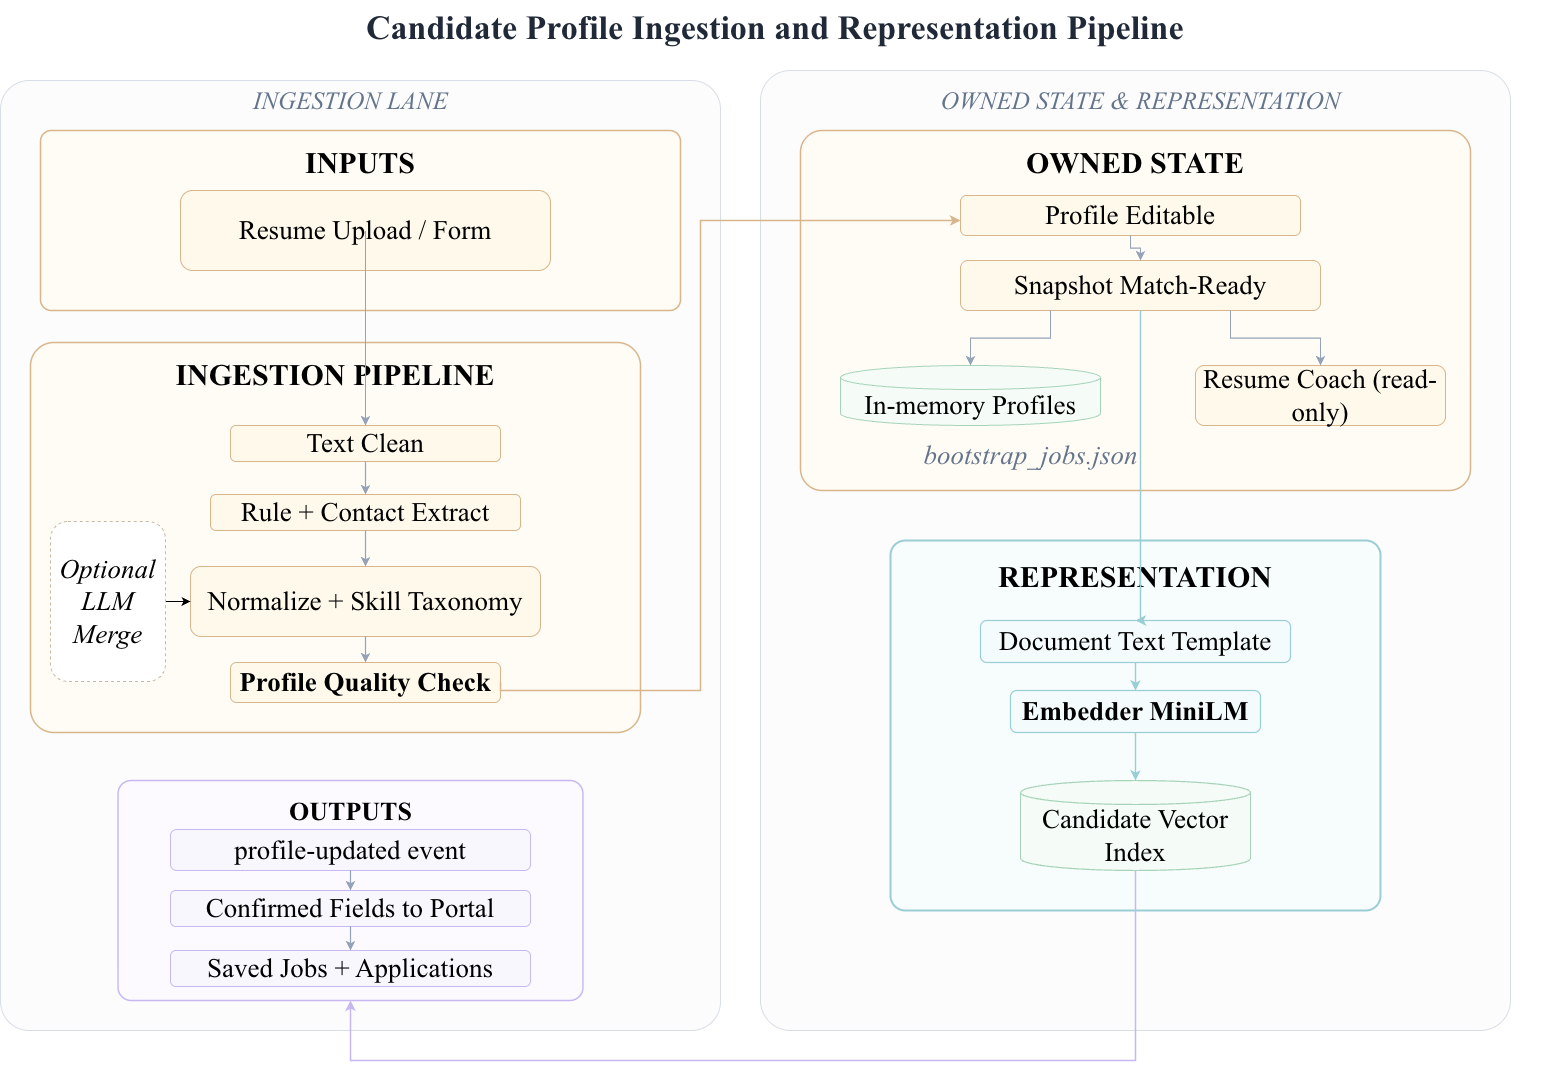
\includegraphics[width=0.95\linewidth]{figures/Fig2.png}
\caption{Candidate-side ingestion and representation pipeline. The candidate-side component owns the editable profile and the versioned snapshot. The ingestion lane accepts a resume upload, runs text clean and rule-based extraction, normalizes the result against the shared skill vocabulary (with an optional LLM fallback for ambiguous fields), and presents the parsed result to the user as a review form. Only on user confirmation does the component register a snapshot and emit a profile-updated event.}
\label{fig:candidate-pipeline}
\end{figure*}

\begin{figure*}[!t]
\centering
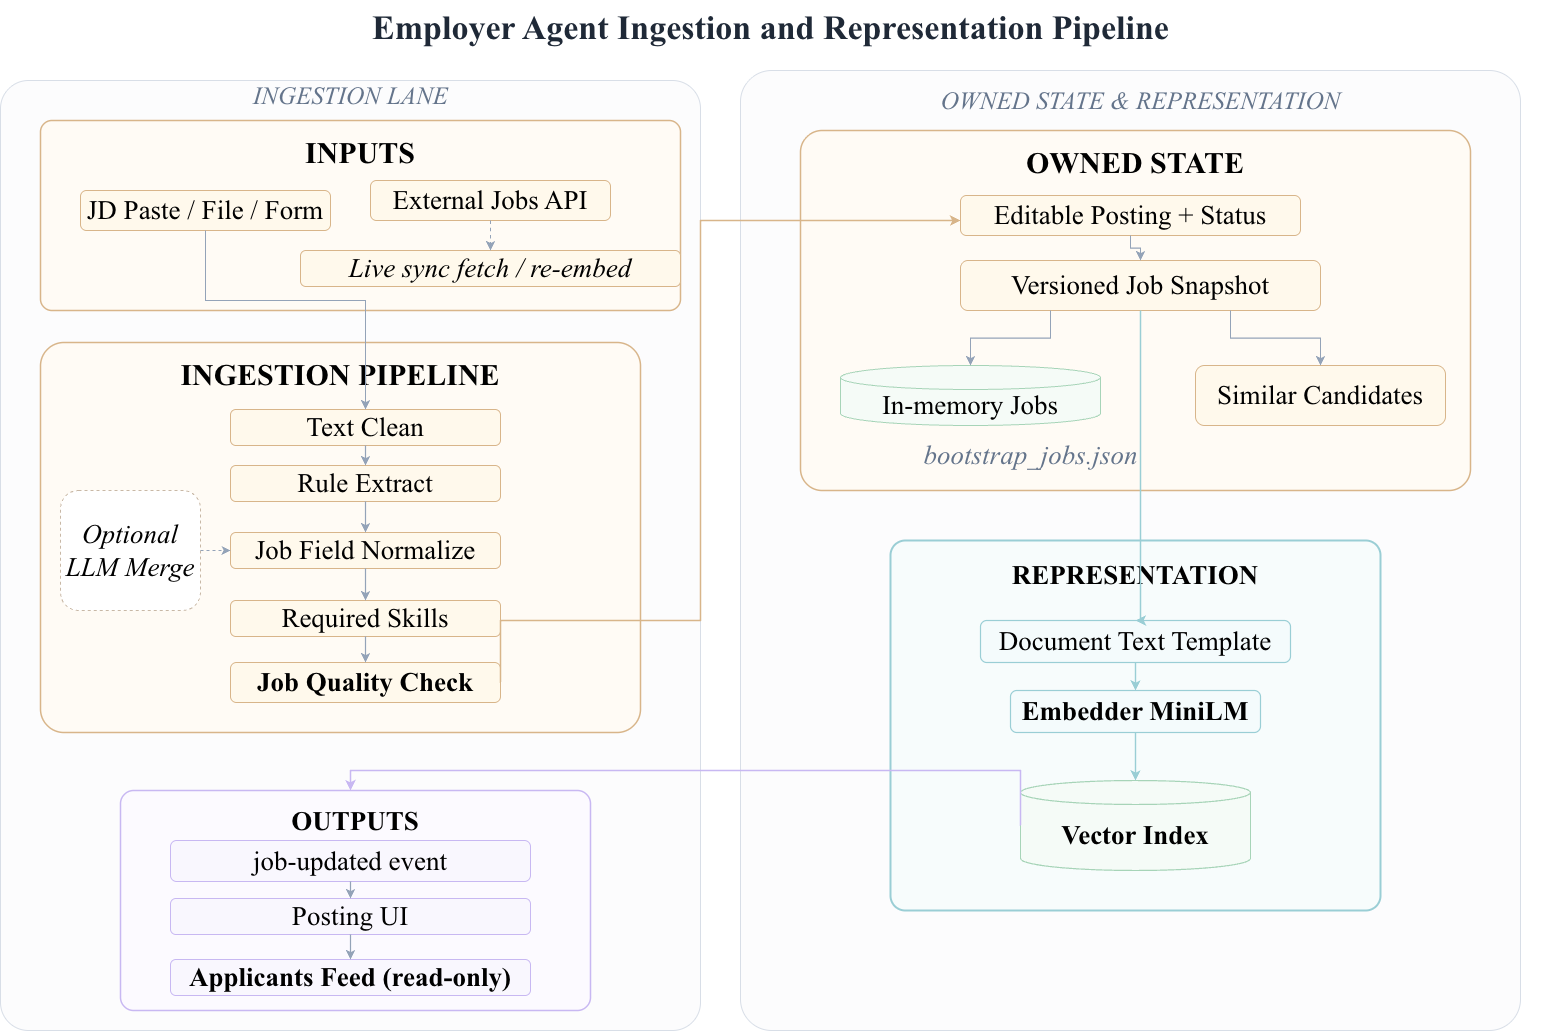
\includegraphics[width=0.95\linewidth]{figures/Fig3.png}
\caption{Employer-side ingestion and representation pipeline. The employer-side component mirrors the candidate-side layout for the job side: editable posting, versioned snapshot, and an ingestion lane that accepts a job description paste, file, or external API and presents the parsed result as a recruiter review form. Only on confirmation does the component register a snapshot and emit a job-updated event.}
\label{fig:employer-pipeline}
\end{figure*}

\begin{figure*}[!t]
\centering
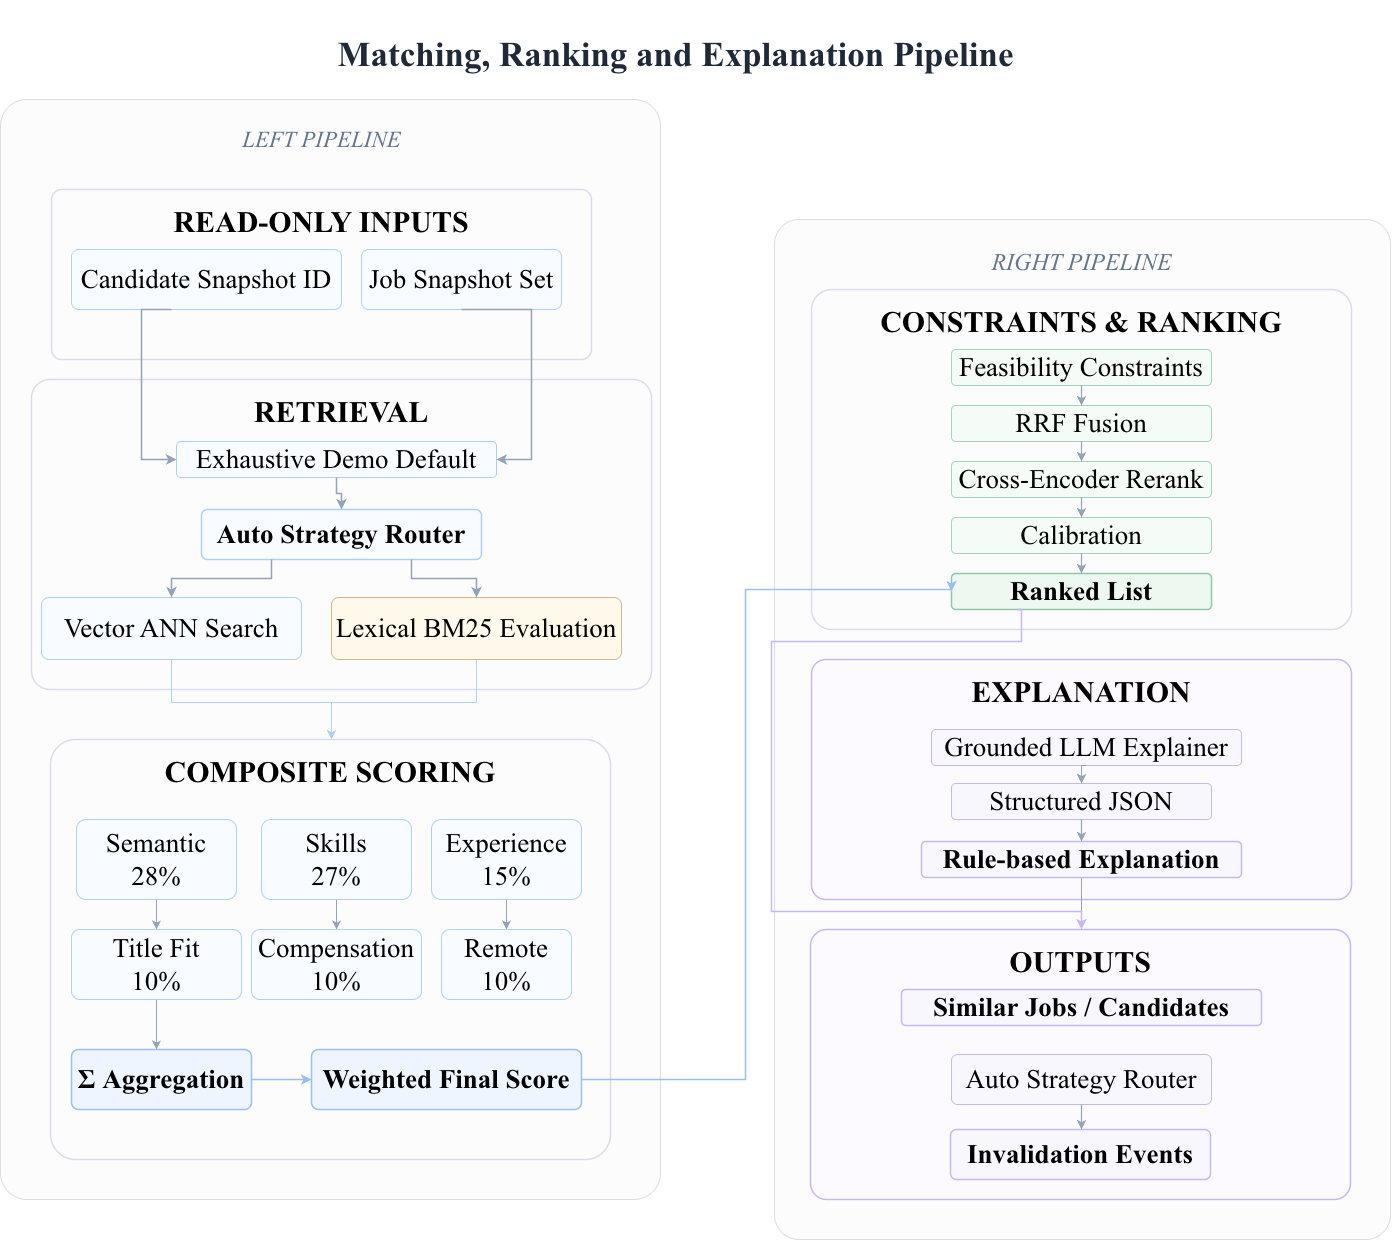
\includegraphics[width=0.95\linewidth]{figures/Fig5.png}
\caption{End-to-end methodology: from resume and job-description inputs through knowledge representation, hybrid retrieval, composite scoring, RRF fusion, cross-encoder rerank, calibration, and component-level explanation, to the ranked, explained, and calibrated output. The dashed feedback arrow indicates that the calibrated confidence is recomputed on each ranking request and used to inform downstream display and user actions. The same pipeline runs for both the candidate-initiated and the employer-initiated direction; the matchmaking component does not see the editable profile behind either side.}
\label{fig:methodology}
\end{figure*}

\subsection{Problem formulation and notation}\label{sec:3.1}
We begin with a formal statement of the task and a description of the notation used throughout the section.
Let $\mathcal{R} = \{r_1, r_2, \ldots, r_n\}$ denote a set of resumes and $\mathcal{J} = \{j_1, j_2, \ldots, j_m\}$ denote a set of job descriptions.
Each resume $r_i$ is parsed into a structured representation $\tilde{r}_i = (S_i, E_i, C_i, P_i)$ where $S_i$ is a multiset of normalized skill tokens, $E_i$ is an experience tier, $C_i$ is a compensation expectation, and $P_i$ is a remote-work preference.
Each job $j_k$ is parsed into a structured representation $\tilde{j}_k = (S_k^{\text{req}}, S_k^{\text{pref}}, E_k^{\min}, E_k^{\max}, C_k, P_k, T_k)$ where $S_k^{\text{req}}$ and $S_k^{\text{pref}}$ are required and preferred skill tokens, $E_k^{\min}$ and $E_k^{\max}$ are the experience bounds, $C_k$ is the compensation band, $P_k$ is the remote-work policy, and $T_k$ is the job title.
The task is to learn a scoring function $f: \mathcal{R} \times \mathcal{J} \to \mathbb{R}$ that ranks the jobs for a given resume, and to produce alongside the ranking a per-decision factor decomposition and a calibrated confidence value.
The factor decomposition is a vector $d(r_i, j_k) \in \mathbb{R}^6$ where the six components correspond to the six channels described in \secref{sec:3.5}, and the calibrated confidence is a value $c(r_i, j_k) \in [0, 1]$ that the user can read as a signal of the system's uncertainty.

\subsection{Methodology at a glance}\label{sec:3.2}
The end-to-end methodology is a six-stage pipeline: inputs (resume or job description, user preferences, and the catalog of normalized skill tokens) flow through knowledge representation, hybrid retrieval, composite ranking, component-level explanation, and confidence calibration before the ranked list, per-channel reasons, and confidence value are returned to the user.
\figref{fig:methodology-flow} visualizes the six stages with the calibrated confidence used only for downstream display alongside the ranked list; the ranking weights themselves are fixed hand-set domain priors, not fitted to the labeled pairs (\secref{sec:3.5}).
The same pipeline is run in both directions (candidate-initiated and employer-initiated) without modification, and the per-direction user interface is the only stage that is direction-specific.
The detailed block architecture, the per-component decomposition, and the per-stage implementation are described in the following subsections.

\begin{figure*}[!t]
\centering
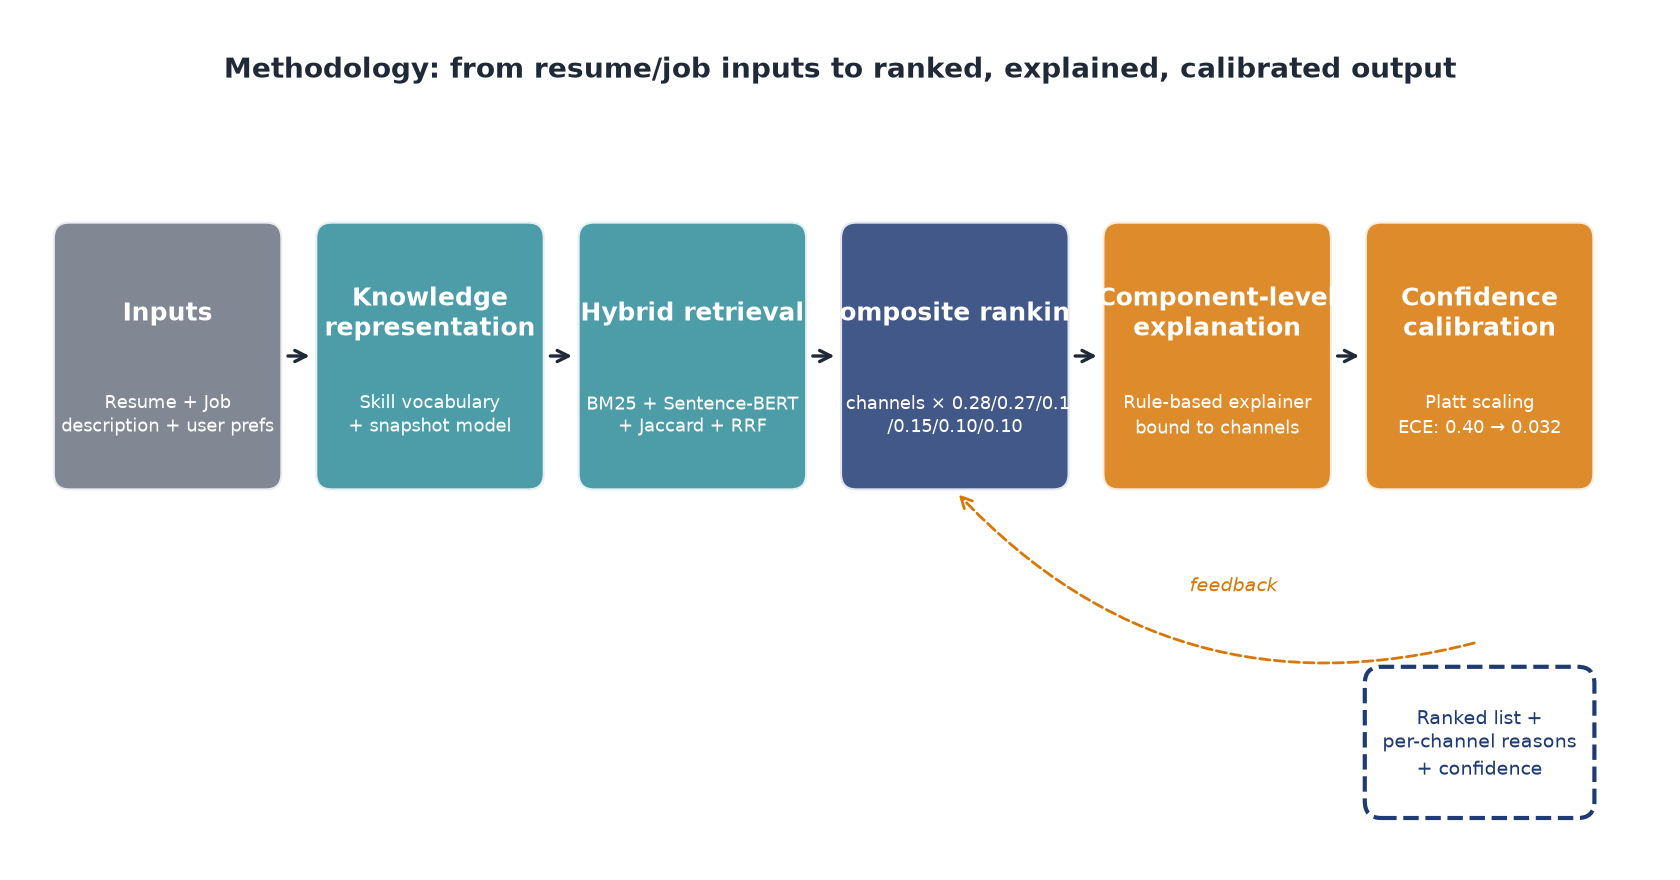
\includegraphics[width=0.85\linewidth]{figures/fig3_methodology_flow.png}
\caption{End-to-end methodology: from resume and job-description inputs through knowledge representation, hybrid retrieval, composite scoring, component-level explanation, and Platt-scaled confidence calibration to the ranked list with per-channel reasons and a calibrated confidence value. The dashed orange feedback arrow indicates that the calibrated confidence is recomputed on each ranking request and is available to inform downstream display and user actions. The same pipeline runs in both the candidate-initiated and the employer-initiated direction; the per-direction portal (Figs.~\ref{fig:app} and~\ref{fig:app2}) is the only stage that is direction-specific.}
\label{fig:methodology-flow}
\end{figure*}

\subsection{Multi-agent system architecture}\label{sec:3.3}
The architecture decomposes the ranking workflow into three cooperating components, each with a single user constituency and a clearly defined interface to the others.
\figref{fig:hld} (introduced in \secref{sec:1}) shows the high-level layout; \figref{fig:arch} below traces the end-to-end matchmaking workflow; \figref{fig:capstone} gives the detailed system architecture with the admin/evaluation console and the data plane.
The role separation is a design-for-accountability choice: the candidate-side component owns the candidate's editable profile and the candidate's read-only snapshot; the employer-side component owns the employer's editable job description and the job's read-only snapshot; the matchmaking component reads both snapshots, scores each pair, attaches the per-decision factor decomposition, and attaches the calibrated confidence.
The role boundary is also the privacy boundary: the candidate-side component does not see the employer's editable job description; the employer-side component does not see the candidate's editable profile; the matchmaking component never writes into either side.
The LLM is used by the candidate-side component for resume parsing and by the matchmaking component for explanation generation; the LLM is not on the hot ranking path.
The hot path must be deterministic, fast, and auditable, and current LLM technology does not meet all three requirements at production scale; placing the LLM on the cold path is a direct consequence of this constraint.
The role-separated layout maps to the privacy boundary in production HR systems.

\begin{figure*}[!t]
\centering
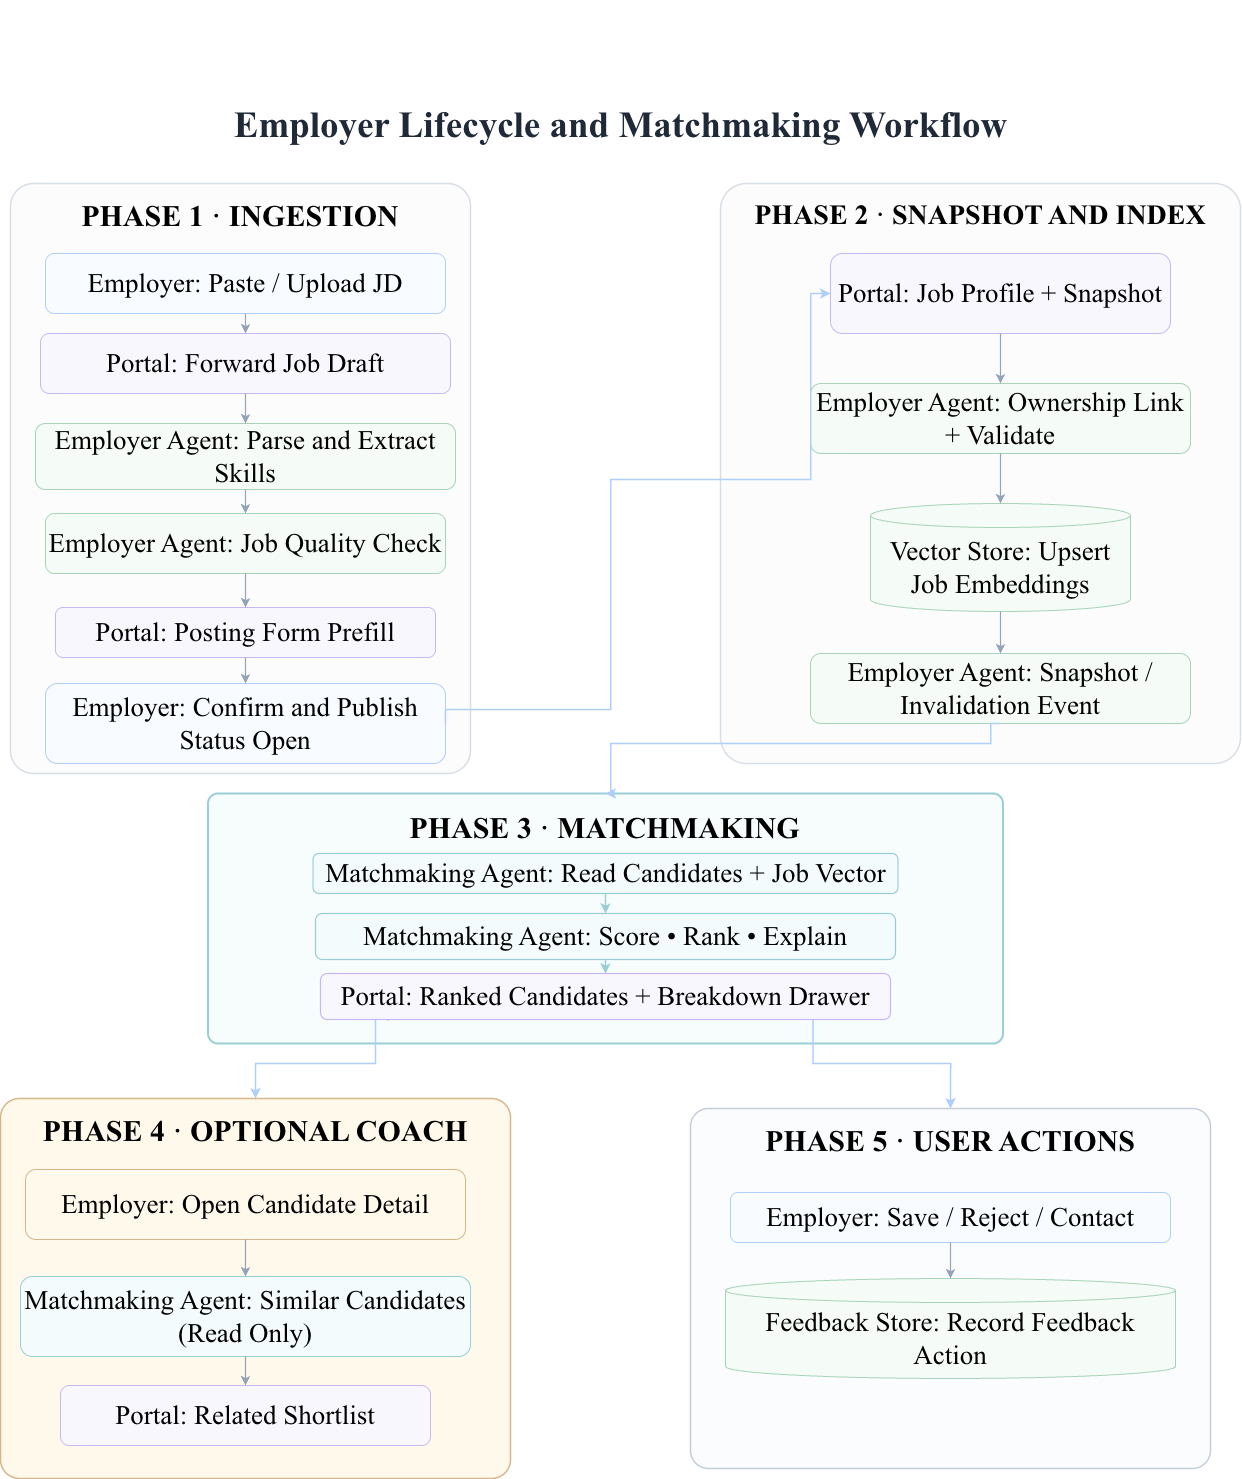
\includegraphics[width=0.88\linewidth]{figures/Fig4.png}
\caption{End-to-end matchmaking workflow (employer direction shown; the candidate direction is symmetric). The workflow is the same whether it is initiated by a candidate refreshing their matches or by an employer refreshing their shortlist: ingestion, snapshot/index, ranking, optional coach feedback, and user actions are sequenced so the read-only matchmaking component never crosses the ownership boundary.}
\label{fig:arch}
\end{figure*}

\begin{figure*}[!t]
\centering
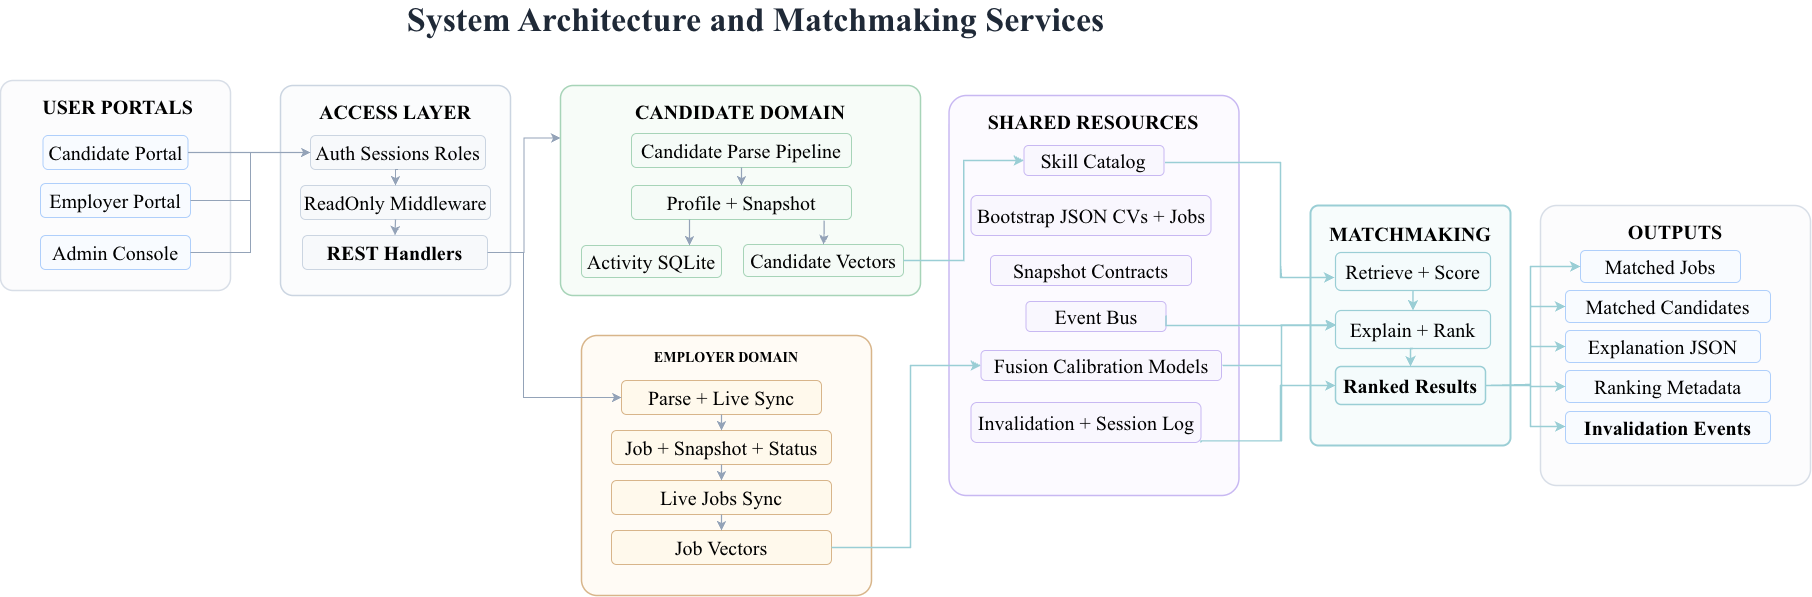
\includegraphics[width=0.95\linewidth]{figures/Fig7.png}
\caption{Detailed system architecture and matchmaking services. The user portals (candidate, employer, admin) sit above an access layer with auth, role, and read-only middleware that fronts the REST handlers. The candidate domain owns the parse pipeline, profile, snapshot, and activity log; the employer domain owns the parse + live sync, job + snapshot, and job vectors. The shared resources layer exposes the skill catalog, bootstrap data, snapshot contracts, event bus, fusion and calibration models, and the invalidation log. The matchmaking component reads from the shared resources and from the snapshot edges of each domain, never from the editable stores.}
\label{fig:capstone}
\end{figure*}

\subsection{Knowledge representation and retrieval}\label{sec:3.4}
The shared knowledge representation is a skill vocabulary $\mathcal{V} = \{v_1, v_2, \ldots, v_V\}$ of $V \approx 5{,}000$ normalized skill tokens with alias mappings from free-text skill descriptions to vocabulary tokens.
Both the candidate-side and the employer-side components consult the same vocabulary; a free-text skill description in a resume or job description is mapped to a vocabulary token by a rule-based normalizer with an LLM fallback for ambiguous cases.
The retrieval layer is a hybrid of four channels:
\emph{(i)} BM25 \citep{robertson1995okapi} over the free-text concatenation of the resume and the job description, with a field-boosted weighting that emphasizes the title field.
\emph{(ii)} Sentence-BERT cosine similarity \citep{reimers2019sentence} over the embedding of the resume's free-text concatenation and the embedding of the job's free-text concatenation, using the \texttt{all-MiniLM-L6-v2} encoder with $d = 384$.
\emph{(iii)} Jaccard skill overlap over the normalized skill multisets, with a soft-embed weighting that allows partial credit for skill aliases (e.g., "ML" and "machine learning" are mapped to the same vocabulary token but "K8s" and "Kubernetes" are partial aliases).
\emph{(iv)} Reciprocal rank fusion \citep{cormack2010reciprocal} of the top-$K$ lists from the three channels above, with $K = 10$ and the RRF constant $k = 60$.
The four channels are evaluated independently and the results are fused by the composite ranking layer described next.
The choice of four channels is motivated by the empirical observation that no single channel dominates across all pairs: BM25 is strong on exact term matches, Sentence-BERT is strong on paraphrases, Jaccard is strong on skill overlap, and RRF is a robust fusion of the three.
The hybrid layer returns, for each pair $(r_i, j_k)$, a four-dimensional vector of channel scores; the composite ranking layer combines the four channels with the two non-retrieval channels (experience, compensation, remote) into a single score.

\subsection{Composite ranking with decomposition}\label{sec:3.5}
The composite ranking layer combines six channels into a single score.
\figref{fig:channels} documents the six channel weights, and the equation below makes the combination explicit.
The two high-weight channels (semantic 0.28 and skill 0.27) carry the dominant share of the score; the four medium- and low-weight channels (title 0.10, experience 0.15, compensation 0.10, remote 0.10) carry the remaining 45\%.
The weights are \emph{hand-set domain priors}, not fitted to the labeled pairs; a bootstrap weight-stability analysis (\secref{sec:5}) confirms they behave as a design prior rather than a validation-optimized optimum, and a protocol-gated search over 25 ranking configurations (\secref{sec:5}) finds no configuration that significantly outperforms this fixed composite on the present corpus.

\begin{figure*}[!t]
\centering
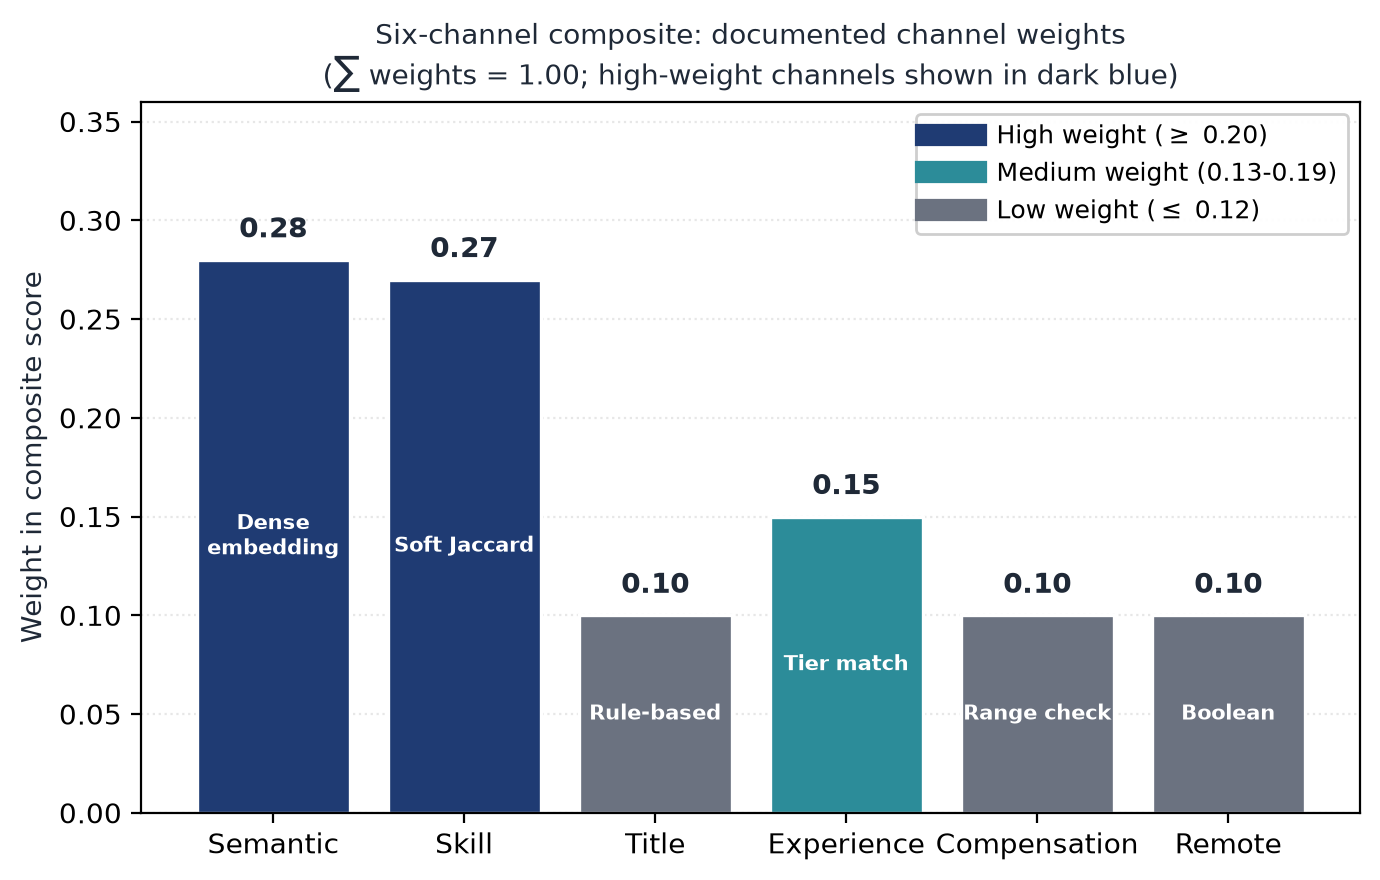
\includegraphics[width=0.95\linewidth]{figures/fig5_channel_contribution.png}
\caption{Six-channel composite: documented channel weights. The two high-weight channels (semantic 0.28 and skill 0.27) carry the dominant share of the score; the four medium- and low-weight channels (title 0.10, experience 0.15, compensation 0.10, remote 0.10) carry the remaining 45\%. The weights are hand-set domain priors (not fitted to the labeled pairs); see the weight-stability analysis in \secref{sec:5}.}
\label{fig:channels}
\end{figure*}

The six channels are:
\emph{(1)} semantic similarity (the Sentence-BERT cosine from the retrieval layer).
\emph{(2)} skill overlap (the Jaccard from the retrieval layer, with the soft-embed weighting).
\emph{(3)} title fit (a binary indicator of whether the resume's most recent title matches the job's title in the same domain, computed by a rule on the title strings).
\emph{(4)} experience tier fit (a function of the difference between the resume's experience tier and the job's experience bounds, with a piecewise-linear penalty for under-qualification and over-qualification).
\emph{(5)} compensation fit (a binary indicator of whether the resume's compensation expectation is within the job's compensation band).
\emph{(6)} remote-work preference fit (a binary indicator of whether the resume's remote-work preference is compatible with the job's remote-work policy).
The six channel scores are combined by a fixed-weight linear combination:
\begin{equation}
\begin{split}
f(r_i, j_k) =\, & 0.28\,s_{\text{sem}} + 0.27\,s_{\text{skill}} + 0.10\,s_{\text{title}} \\
               & + 0.15\,s_{\text{exp}} + 0.10\,s_{\text{comp}} + 0.10\,s_{\text{remote}}
\end{split}
\end{equation}
where the weights are hand-set domain priors (not fitted to the labeled pairs) and are reported as part of the system configuration; \secref{sec:5} reports a bootstrap stability analysis and a protocol-gated configuration search that together justify retaining this fixed, auditable prior.
The choice of a fixed-weight composite is motivated by two engineering properties: the per-decision factor decomposition is exact (the channel scores are reported in the explanation panel), and the composite is auditable (the weights are documented and the calibration is reported on the same composite).

\emph{Relation-aware graded skill matcher.} The default skill channel (2) uses binary Jaccard overlap, which gives all-or-nothing credit. As an auditable alternative we define a graded, relation-aware matcher that resolves each (candidate skill, required skill) pair to one of three relation classes and aggregates by coverage: for each required skill we take the best credit over the candidate's skills --- $1.0$ if they share a canonical form after synonym/abbreviation/orthographic normalization (\textsc{exact}), $0.5$ if they fall in the same skill-taxonomy group (\textsc{related}), and $0$ otherwise (\textsc{unrelated}) --- and average over the required skills. The credits are fixed a priori (not fitted to any evaluation), and \textsc{related} never receives \textsc{exact}-level credit. Unlike symmetric Jaccard this form is coverage-oriented (how well the candidate covers the job's stated requirements) and awards partial, never full, credit to related-but-not-identical skills. \secref{sec:5.7} evaluates this matcher on a de-circularized skill-pair benchmark and, holding all weights fixed, decomposes its ranking effect into the coverage-form change and the relation-aware credit; the primary composite retains binary Jaccard for comparability with the baselines, and the graded matcher is reported as an auditable enhancement rather than adopted as the headline configuration.
A learned logistic-regression fusion is reported as an alternative in the offline evaluation; the learned fusion ties the best single configuration but is fit on the same labeled pairs it is judged against, which is an overfitting risk (see \secref{sec:6}).

\subsection{Component-level explanation generation}\label{sec:3.6}
The component-level explanation is generated by a rule-based explainer that is bound to the same six channels that produce the score.
For each channel that contributes more than a configured threshold (default: 5\% of the composite score), the explainer emits a bullet that names the channel and the value that drove the contribution.
For example, if the skill-overlap channel contributes 0.27 to the composite and the overlap is on the "Python" and "machine learning" skills, the bullet is "Matched on Python and machine learning (skill overlap 0.27)."
If the experience-tier channel contributes 0.05 because the resume's experience tier is below the job's lower bound, the bullet is "Below the experience bound by one tier (experience fit 0.05)."
The bullets are produced deterministically from the channel scores and the structured representations; the explanation is consistent with the score by construction.
An LLM-based explainer is reported as a comparison in the offline evaluation; the LLM-based explainer is a GPT-class model prompted with the channel scores and the structured representations, and the natural-language rationale is generated by the LLM.
The trade-off is that the LLM-based explainer has higher skill-mention coverage (it names a concrete skill in roughly half of the bullets) but lower faithfulness (some bullets are inconsistent with the channel scores because the LLM hallucinates a contribution that the channels did not produce).
The rule-based explainer is the default in the prototype; the LLM-based explainer is reported in the offline evaluation as a comparison.

\subsection{Confidence calibration}\label{sec:3.7}
The composite ranking output is a score in $\mathbb{R}$, and the prototype system displays a confidence value in $[0, 1]$ alongside the score.
The mapping from score to confidence is learned by Platt scaling \citep{platt1999probabilistic,guo2017calibration,lofstrom2024calibrated} on a held-out calibration set of 21 strong and 26 partial labels.
The use of Platt scaling for ranking-system calibration follows the calibrated-explanations framework \citep{lofstrom2024calibrated}, which provides uncertainty information alongside rule-based explanations; here it is applied, in standard form, to the scalar composite score, and we make no novelty claim for the calibration mechanism itself (see \secref{sec:2} and the trade-off analysis in \secref{sec:5}).
The Platt scaling parameters are a slope $a$ and an intercept $b$, applied to the composite score:
\begin{equation}
c(r_i, j_k) = \sigma(a \cdot f(r_i, j_k) + b)
\end{equation}
where $\sigma$ is the logistic sigmoid.
The calibration parameters are learned by maximum likelihood on the calibration set; the calibration quality is reported as the expected calibration error (ECE), the Brier score, and a reliability diagram that plots the predicted confidence against the empirical relevance rate over all judged (resume, job) pairs under the held-out 5-fold protocol (\secref{sec:4}).
The uncalibrated composite has ECE = 0.40, which is too poorly calibrated to display directly; the calibrated composite has held-out 5-fold ECE = 0.019, a large reduction, though the calibrated confidence has low discrimination near the base rate (\secref{sec:5.3}).
The Brier score of the calibrated system is 0.093.
The Platt parameters are exposed in the system configuration; a sensitivity analysis on the parameters is reported in \secref{sec:5}.

\subsection{Implementation details}\label{sec:3.8}
The system is implemented as a small web stack: a Python backend for the parsing, retrieval, ranking, calibration, and explanation logic, and a Node frontend for the candidate, employer, and administrator portals.
The system is reproducible from a clean clone: a single command runs the regression benchmark and reproduces the reported numbers within a $\pm 0.04$ nDCG tolerance.
The test suite is 302 Python unit tests and 39 Node tests, for a total of 341 tests; the CI gate fails the build on a regression greater than the tolerance.
The latency profile is reported in \secref{sec:5}: the composite bi-encoder completes in approximately 0.4 ms per query, the cross-encoder completes in approximately 141.7 ms per query, and the end-to-end request (including the rule-based explainer) completes in under 10 ms per request.
The LLM-based explainer is invoked only when the user requests a natural-language rationale, and is gated by a per-request budget; the typical invocation cost is below the cost of the ranking itself.
The prototype, the frozen demo corpus, the synthetic corpus and generator, the evaluation scripts, the explanation generator, the calibration layer, and the regression benchmark are released as an open-source artifact (to be deposited with a citable DOI upon acceptance; see the data availability statement at the end of this paper).

\subsection{Engineering surface and integration}\label{sec:3.9}
The engineering surface of the system is reported here in the level of detail required for a deployment team to reproduce the deployed claims and to integrate the prototype with an existing ATS.
The Python backend is structured as a small set of modules: a \texttt{parser} module for resume and job description ingestion, a \texttt{retrieval} module for the four retrieval channels, a \texttt{ranking} module for the composite scoring, an \texttt{explanation} module for the rule-based and LLM-based explainers, and a \texttt{calibration} module for the Platt scaling and the reliability-diagram computation.
Each module has a typed interface and a unit-test suite; the modules are independently deployable, and a deployment team can swap a module (e.g., replace the rule-based explainer with a deployment-specific template) without touching the other modules.
The Node frontend is structured as three single-page applications (candidate, employer, administrator) that share a common API client; the frontend has 39 unit tests that cover the API client and the form-validation logic.
The integration with an existing ATS is via a documented REST API: the ATS sends a parsed resume and a job description to the system, the system returns the ranked list, the per-decision factor decomposition, the calibrated confidence, and the explanation; the ATS renders the response in its own UI.
As an \emph{illustrative} engineering estimate derived from the prototype architecture (not from a measured production deployment), a typical integration might be on the order of 200--300 engineering hours, of which 50--100 hours are infrastructure engineering (Kubernetes deployment, monitoring, logging) and 20--40 hours per month are ongoing maintenance (model retraining, calibration updates, explanation-template updates).
The latency budget (under 10 ms per end-to-end request) means that the prototype can be deployed behind an existing ATS without changing the user-facing latency budget; the LLM-based explainer is invoked only on user request and is gated by a per-request budget to prevent cost overruns.

\begin{figure*}[!t]
\centering
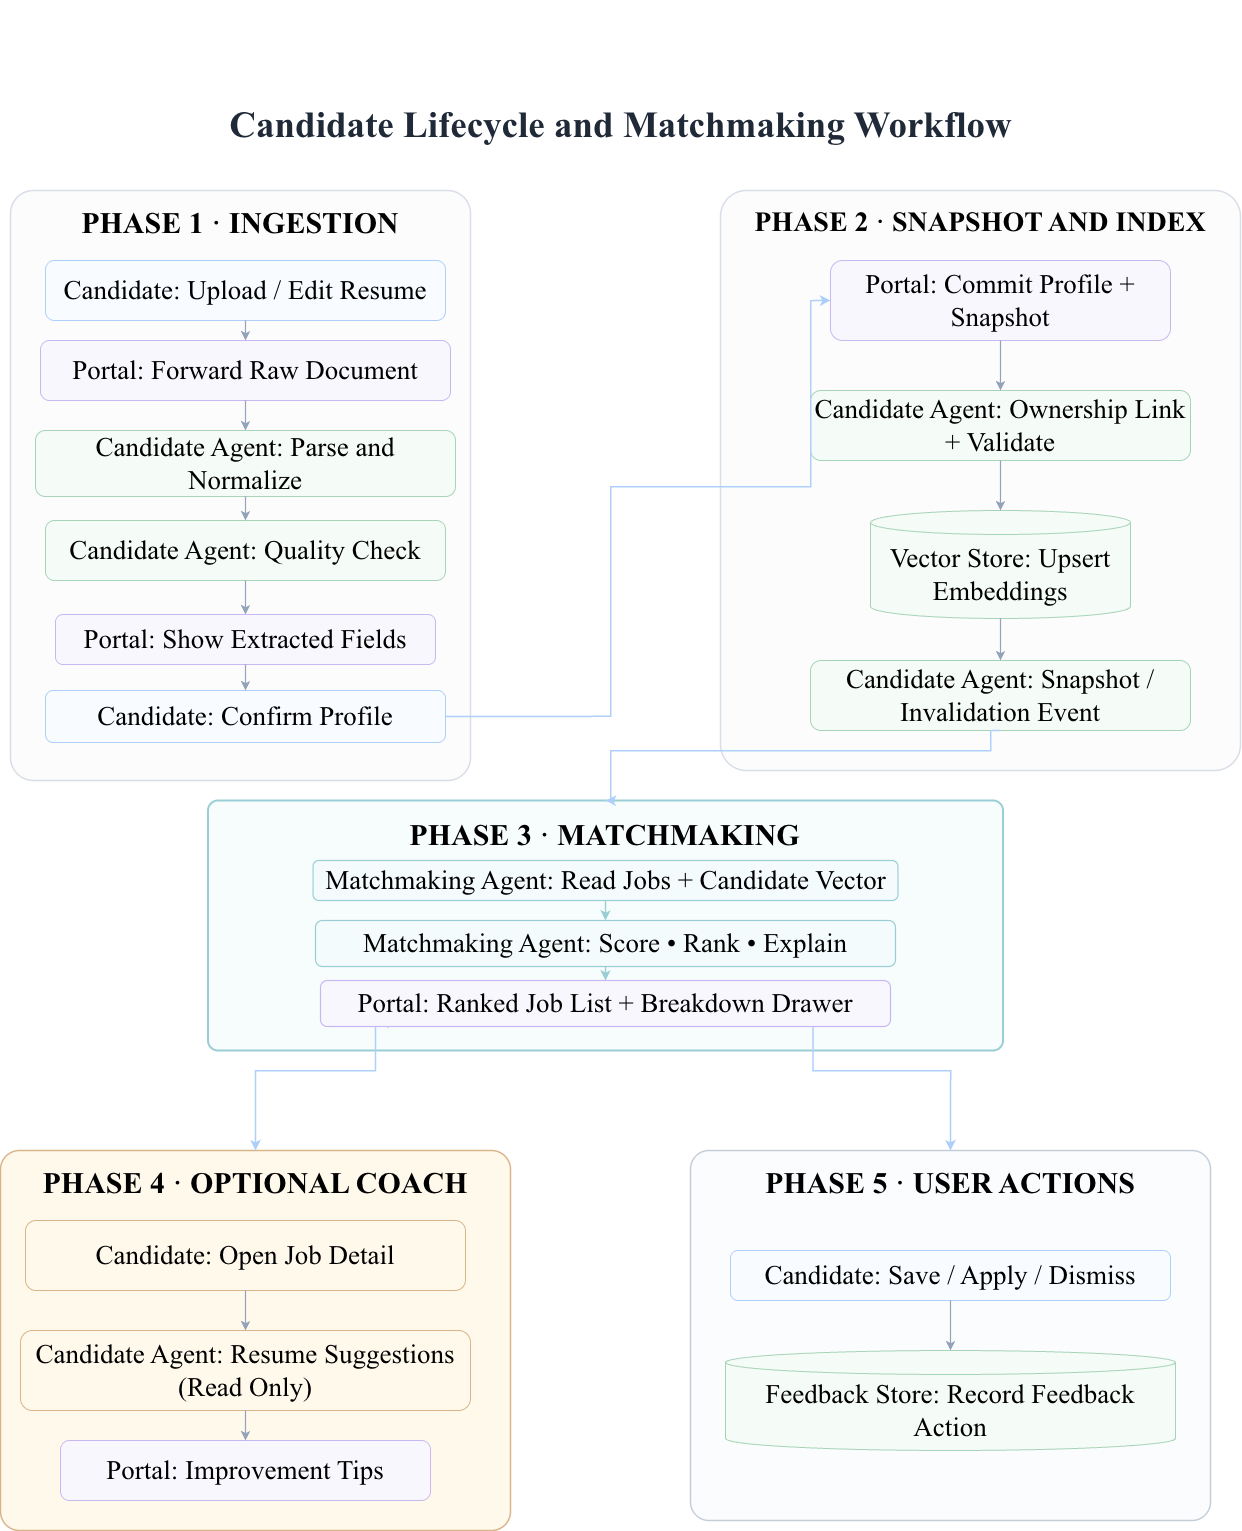
\includegraphics[width=0.95\linewidth]{figures/Fig6.png}
\caption{Candidate-side lifecycle and matchmaking workflow. The end-to-end candidate journey is: (1) ingestion of the resume and confirmation of the parsed profile, (2) snapshot registration and vector upsert, (3) matchmaking, (4) optional resume-coach feedback (read-only suggestions for the next edit), and (5) user action (save, apply, or dismiss). The matchmaking component is invoked between step 2 and step 5; the optional coach is invoked only on user request and is gated by a per-request budget.}
\label{fig:candidate-lifecycle}
\end{figure*}

\subsection{Cross-encoder diagnosis}\label{sec:3.10}
The cross-encoder reranker, evaluated in \secref{sec:5.1}, does not improve on the fixed composite (nDCG@5 0.939 vs 0.949) on the frozen demo corpus despite roughly 340$\times$ the latency.
The diagnosis is twofold.
\emph{(i) Small training set.} The cross-encoder is trained on the same 47 labeled pairs that are used for the offline evaluation; with a bi-encoder baseline at nDCG 0.949, the cross-encoder overfits to the residual errors of the bi-encoder rather than learning a robust re-ranking function.
A larger training set (the larger-corpus study mentioned in \secref{sec:7}) would reduce the overfitting risk, but is not yet available.
\emph{(ii) Latency.} The cross-encoder is approximately 340$\times$ slower than the bi-encoder (141.7 ms vs.\ 0.4 ms per query); the latency cost is incompatible with the hot ranking path of a high-throughput ATS.
The diagnosis motivates the engineering decision to disable the cross-encoder by default in the prototype and to report the cross-encoder result in the offline evaluation for completeness.
A future-work direction is to train a lightweight cross-encoder on a larger corpus and to evaluate the latency--quality trade-off at production scale; the present system does not include this direction.
The cross-encoder-disable decision is documented in the released benchmark JSON.
